\documentclass[paper=a4, fontsize=11pt]{scrartcl}
\usepackage[T1]{fontenc}
\usepackage{fourier}

\usepackage[english]{babel}															% English language/hyphenation
\usepackage[protrusion=true,expansion=true]{microtype}	
\usepackage{amsmath,amsfonts,amsthm} % Math packages
\usepackage[pdftex]{graphicx}	
\usepackage{url}
\usepackage{hyperref}


%%% Custom sectioning
\usepackage{sectsty}
\allsectionsfont{\centering \normalfont\scshape}
\usepackage{subfigure}

\usepackage{comment}


%%% Custom headers/footers (fancyhdr package)
\usepackage{fancyhdr}
\pagestyle{fancyplain}
\fancyhead{}											% No page header
\fancyfoot[L]{}											% Empty 
\fancyfoot[C]{}											% Empty
\fancyfoot[R]{\thepage}									% Pagenumbering
\renewcommand{\headrulewidth}{0pt}			% Remove header underlines
\renewcommand{\footrulewidth}{0pt}				% Remove footer underlines
\setlength{\headheight}{13.6pt}


%%% Equation and float numbering
%\numberwithin{equation}{section}		% Equationnumbering: section.eq#
%\numberwithin{figure}{section}			% Figurenumbering: section.fig#
%\numberwithin{table}{section}				% Tablenumbering: section.tab#


%%% Maketitle metadata
\newcommand{\horrule}[1]{\rule{\linewidth}{#1}} 	% Horizontal rule

\title{
		%\vspace{-1in} 	
		\usefont{OT1}{bch}{b}{n}
		\normalfont \normalsize \textsc{CS650 - Computer Vision} \\ [25pt]
		\horrule{0.5pt} \\[0.4cm]
		\huge Programming Lab 3 \\ Graph-cut Segmentation \\
		\horrule{2pt} \\[0.5cm]
}
\author{
		\normalfont 								\normalsize
        Daqing Yi\\[-3pt]		\normalsize
        \today
}
\date{}


%%% Begin document
\begin{document}
\maketitle

\section{Introduction}

A graph cut separates the vertices of a graph into two disjoint subsets.
The minimum cut is one type of graph cuts that uses the smallest number of edges.
The problem can also be reduced to a maximum flow problem by the max-flow min-cut theorem~\cite{wiki:Max-flow_min-cut_theorem}.
By defining the source and the sink in a graph structure, the minimum cut can be used to solve the classification problem that minimizes a given energy function.

In a binary labeling problem, the pixels of an image should be labeled into either foreground or background.
By this way, the foreground object can be extracted from the image.
After defining the source and the sink, we can construct a graph structure that represents both the inter-relationship between neighboring pixels and the likelihoods to be foreground and background.
The minimum cut operation can segment the pixels into foreground and background which minimizes the energy function defined from the weighted edges of the graph structure~\cite{937505}.

In this lab, the code is written in C++.
Qt4.8 is used for the implement of GUI interaction.
The Vladimir Kolmogorov's C++ Implementation ( \emph{ maxflow-v3.03.src } ) is chosen for doing minimum cut.

\section{Graph Cut Segmentation}

The energy function defined for an image is~\cite{rother2004grabcut} 
\begin{equation}
\label{eq:gibbs_energy}
E(\alpha, \theta, z) = U( \alpha, \theta, z ) + V(\alpha, z),
\end{equation} 
where
\begin{equation}
\label{eq:region_energy}
U( \alpha, \theta, z ) = \sum_{n} - \log h( z_{n} ; \alpha_{n} )
\end{equation}
and
\begin{equation}
\label{eq:boundary_energy}
V(\alpha, z) = \gamma \sum_{ (m, n) \in C } dis(m, n)^{-1} [\alpha_{n} \neq \alpha_{m} ] e^{ - \beta (z_{m} - z_{n})^{2} }.
\end{equation}
$ \beta $ is obtained by 
\begin{equation}
\beta = (2 E( (z_{m} - z_{n})^{2} ) )^{-1}.
\end{equation} 
$ U( \alpha, \theta, z ) $ shows the region information, which is determined by the fit of $ \alpha $ to $ z $.
$ V(\alpha, z) $ shows boundary/edge information, which is a smoothness term.
The segmentation can be generated by a global minimum
\begin{equation}
\hat{ \alpha } = \arg \min_{\alpha} E(\alpha, \theta, z).
\end{equation}

Foreground seeds and background seeds are selected by human labeling.
They are used as foreground samples and background samples to train kernel density estimators for foreground and background respectively.
Figure \ref{fig:graph_cut:01} shows a process of graph-cut segmentation.

% Smoothness Ratio 50
% Kernel Density Estimator Bandwidth 80
\begin{figure}[h]
\centering
\subfigure[Origin]{
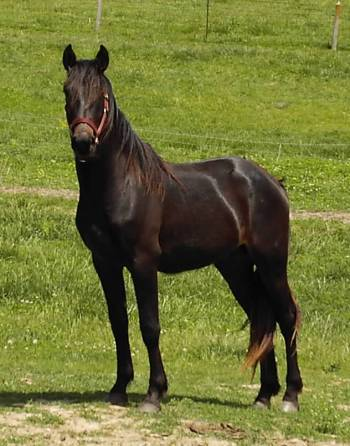
\includegraphics[width=.23\textwidth]{./figure/horse.jpg}
\label{fig:graph_cut:01:origin} }
\subfigure[Labeling]{
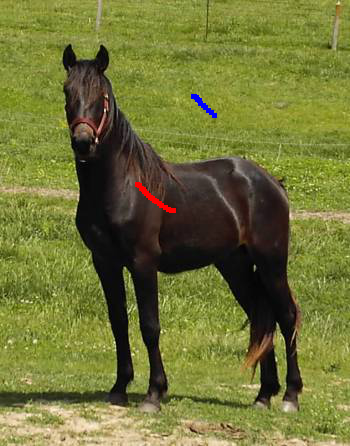
\includegraphics[width=.23\textwidth]{./figure/horse-label.png} 
\label{fig:graph_cut:01:labeling} }
\subfigure[Foreground mask]{

\includegraphics[width=.23\textwidth]{./figure/horse-mask.png} 
\label{fig:graph_cut:01:foreground_mask} }
\subfigure[Foreground cutted]{
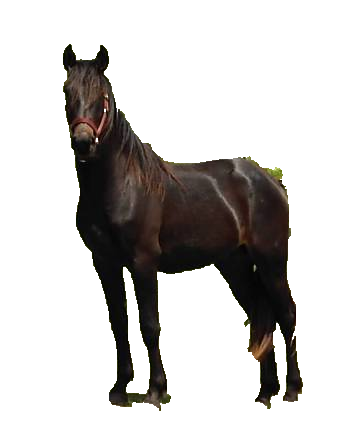
\includegraphics[width=.23\textwidth]{./figure/horse-foreground.png}
\label{fig:graph_cut:01:foreground} }
\caption{Graph cut segmentation on \emph{horse.jpg}.}
\label{fig:graph_cut:01}
\end{figure}

In Equation \eqref{eq:boundary_energy}, $ \gamma $ determines the strength of the boundary energy $ V(\alpha, z) $.
Increasing the parameter $ \gamma $ can strengthen the connectivity relationship between the neighboring pixels.
Thus, more foreground region can be detected.
Figure \ref{fig:graph_cut:02} gives an example.
From Figure \ref{fig:graph_cut:02:less_smooth} to Figure \ref{fig:graph_cut:02:more_smooth}, the parameter $ \gamma $ is increased.

\begin{figure}[h]
\centering
\subfigure[Labeling]{
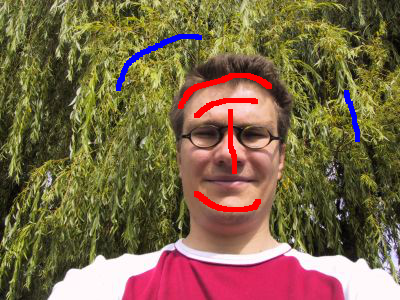
\includegraphics[width=.23\textwidth]{./figure/carsten-label.png}
\label{fig:graph_cut:02:labeling} }
\subfigure[Foreground 1]{

\includegraphics[width=.23\textwidth]{./figure/carsten-foreground2.png} 
\label{fig:graph_cut:02:less_smooth} } % smooth ratio 25
\subfigure[Foreground 2]{

\includegraphics[width=.23\textwidth]{./figure/carsten-foreground1.png} 
\label{fig:graph_cut:02:normal_smooth} } % smooth ratio 50
\subfigure[Foreground 3]{
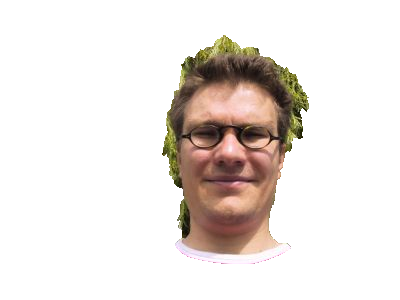
\includegraphics[width=.23\textwidth]{./figure/carsten-foreground3.png}
\label{fig:graph_cut:02:more_smooth} }  % smooth ratio 120
\caption{Graph cut segmentation on \emph{carsten.jpg}.}
\label{fig:graph_cut:02}
\end{figure}

Two types of density estimators are implemented, which are \emph{kernel density estimator} and \emph{Gaussian mixture model}.
The kernel density estimator~\cite{wiki:Kernel_density_estimation} is written as
\begin{equation}
\label{eq:kde}
\hat{f}_{h}(x) = \frac{1}{nh} \sum_{i=1}^{n} K(\frac{x-x_{i}}{h}).
\end{equation}
While the Gaussian mixture model~\cite{wiki:Mixture_model} is written as
\begin{equation}
\hat{f} (x) = \sum_{i=1}^{M} \omega_{i} g(x \mid \mu_{i} , \Sigma_{i})
\end{equation}
and
\begin{equation}
g(x \mid \mu_{i} , \Sigma_{i}) = \frac{1}{(2 * \pi)^{D/2} | \Sigma_{i} |^{1/2} } \exp \{ - \frac{1}{2} (x - \mu_{i})^{T} \Sigma_{i}^{-1} (x-\mu_{i})  \}.
\end{equation}
One of the disadvantage of the kernel density estimator is that the performance depends on the selection of $ h $, especially the sample number is large and the samples are diverse.
The k-means clustering for a Gaussian mixture model is expected to have better performance in this case.
Figure \ref{fig:graph_cut:03} illustrates an example.
Using same parameters, the result by using kernel density estimator is given in Figure \ref{fig:graph_cut:03:kde} and the result by using Gaussian mixture model is given in Figure \ref{fig:graph_cut:03:gmm}.

\begin{figure}[h]
\centering
\subfigure[Labeling]{
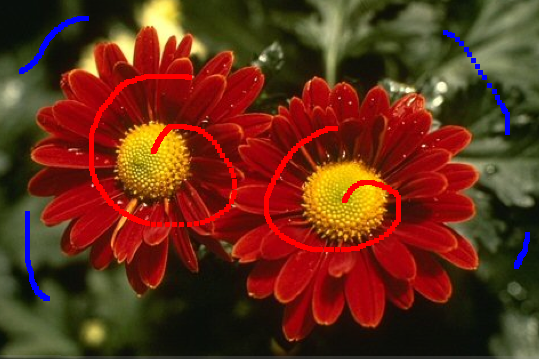
\includegraphics[width=.3\textwidth]{./figure/flowers-label.png}
\label{fig:graph_cut:03:labeling} }
\subfigure[Foreground using KDE]{
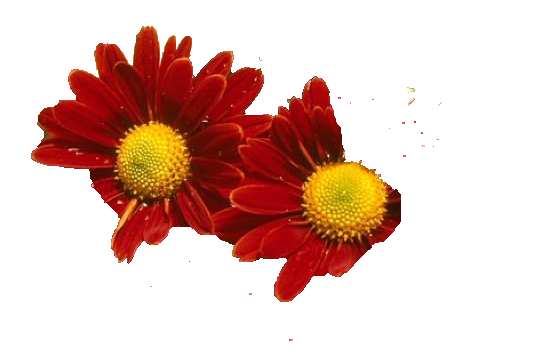
\includegraphics[width=.3\textwidth]{./figure/flowers-foreground1.png} 
\label{fig:graph_cut:03:kde} } % smooth ratio 25
\subfigure[Foreground using GMM]{
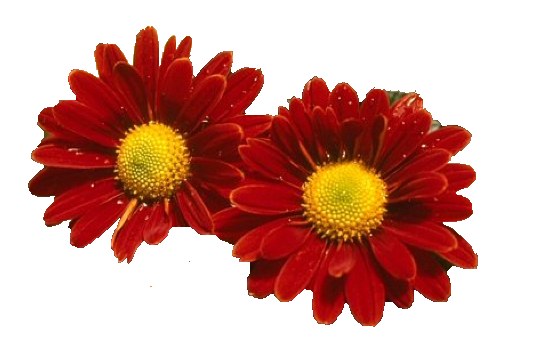
\includegraphics[width=.3\textwidth]{./figure/flowers-foreground2.png} 
\label{fig:graph_cut:03:gmm} } % smooth ratio 50
\caption{Graph cut segmentation on \emph{flowers.png}.}
\label{fig:graph_cut:03}
\end{figure}

\section{Grab Cut Segmentation}

Grab cut is introduced in \cite{rother2004grabcut}.
The foreground seeds and background seeds are initialized by a drawn box.
Then an iterative graph cut is applied till no change appears.
Figure \ref{fig:grab_cut:01} gives the process.
The seeds are initialized firstly from a drawn box in Figure \ref{fig:grab_cut:01:labeling} and Figure \ref{fig:grab_cut:01:seed_vis}.
Then the grab cut can extract the foreground as in Figure \ref{fig:grab_cut:01:foreground}.

 
\begin{figure}[h]
\centering
\subfigure[Labeling]{
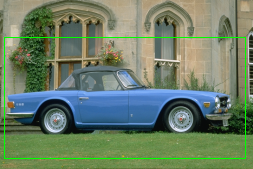
\includegraphics[width=.23\textwidth]{./figure/blue_car-label.png}
\label{fig:grab_cut:01:labeling} }
\subfigure[Seeds distribution]{
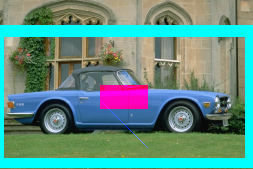
\includegraphics[width=.23\textwidth]{./figure/blue_car-seedVis.png} 
\label{fig:grab_cut:01:seed_vis} } % smooth ratio 25
\subfigure[Foreground mask]{

\includegraphics[width=.23\textwidth]{./figure/blue_car-mask.png} 
\label{fig:grab_cut:01:mask} } % smooth ratio 50
\subfigure[Foreground cutted]{
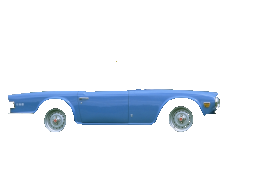
\includegraphics[width=.23\textwidth]{./figure/blue_car-foreground.png}
\label{fig:grab_cut:01:foreground} }  % smooth ratio 120
\caption{Grab cut segmentation on \emph{blue\_car.jpg}. }
\label{fig:grab_cut:01}
\end{figure}

\begin{figure}[h]
\centering
\subfigure[ \emph{food.png} - Label ]{
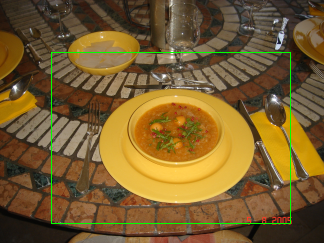
\includegraphics[width=.23\textwidth]{./figure/food-label.png}
\label{fig:grab_cut:02:food} }
\subfigure[ \emph{food.png} - Foreground ]{
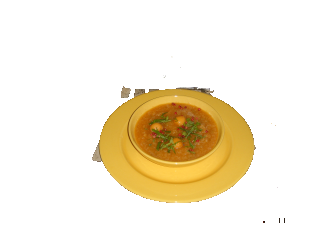
\includegraphics[width=.23\textwidth]{./figure/food-foreground.png} 
\label{fig:grab_cut:02:food_foreground} } % smooth ratio 25
\subfigure[ \emph{fish.png} - Label ]{
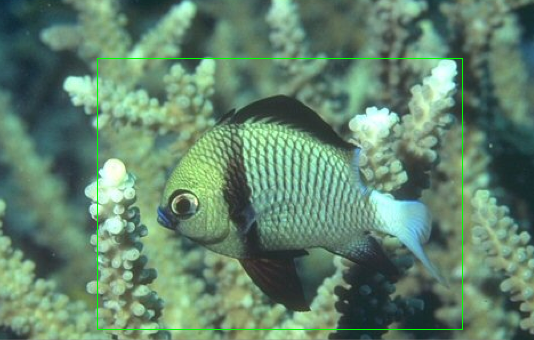
\includegraphics[width=.23\textwidth]{./figure/fish-label.png} 
\label{fig:grab_cut:02:fish} } % smooth ratio 50
\subfigure[ \emph{fish.png} - Foreground ]{
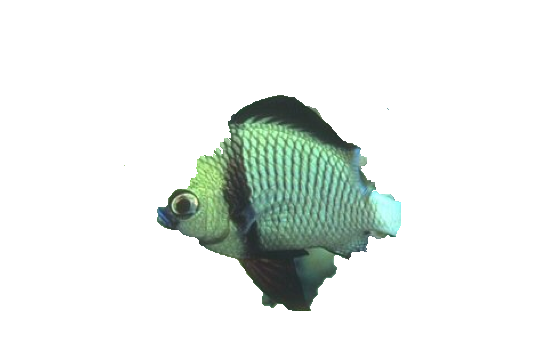
\includegraphics[width=.23\textwidth]{./figure/fish-foreground.png}
\label{fig:grab_cut:02:fish_foreground} }  % smooth ratio 120
\caption{ Comparing the performance on different cases in grab cut. }
\label{fig:grab_cut:02}
\end{figure}


\begin{comment}
As before, prepare a write-up that describes your work.
Show examples of your code applied to different images.
What kinds of images does graph-cut segmentation (or Grab Cut respectively) work well for?
What kinds of images do you find it struggles with? 
\end{comment}

\section{Summary}

RGB color is used to measure the similarity (distance) between different pixels.
If the foreground pixels have similar color with the background pixels, the foreground pixels will be hard to be extracted.
Figure \ref{fig:grab_cut:02} provides an example.
In Figure \ref{fig:grab_cut:02:food}, the foreground object ``plate'' has a strong contrast with the background, it can be easily extracted.
When the foreground object cannot be simply discriminated from the background, the graph cut cannot well find out the foreground object, as it is shown in Figure \ref{fig:grab_cut:02:fish_foreground}.

\begin{figure}[h]
\centering
\subfigure[ \emph{llama.bmp} - Label 1 ]{
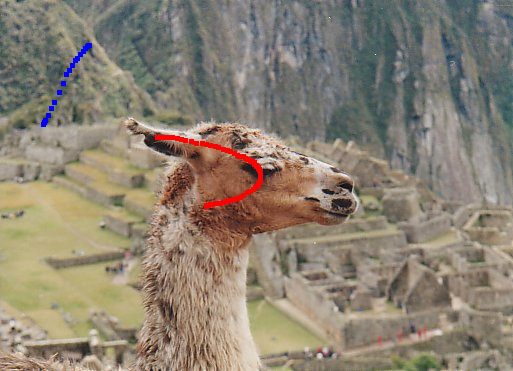
\includegraphics[width=.23\textwidth]{./figure/llama-label1.png}
\label{fig:graph_cut:05:labeling1} }
\subfigure[ \emph{llama.bmp} - Foreground 1 ]{
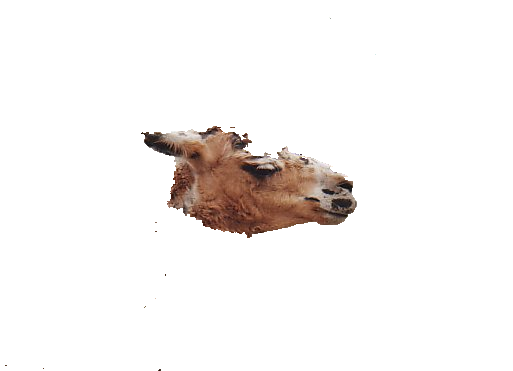
\includegraphics[width=.23\textwidth]{./figure/llama-foreground1.png} 
\label{fig:graph_cut:05:foreground1} } % smooth ratio 25
\subfigure[ \emph{llama.bmp} - Label 2 ]{
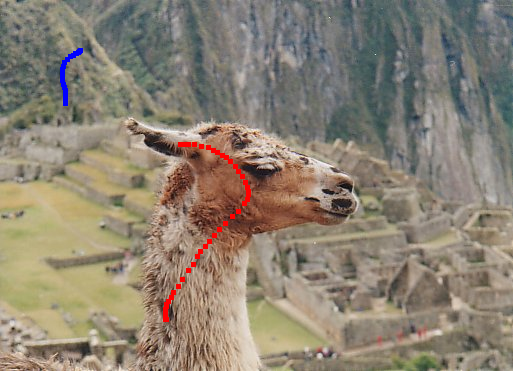
\includegraphics[width=.23\textwidth]{./figure/llama-label2.png} 
\label{fig:graph_cut:05:labeling2} } % smooth ratio 50
\subfigure[ \emph{llama.bmp} - Foreground 2 ]{
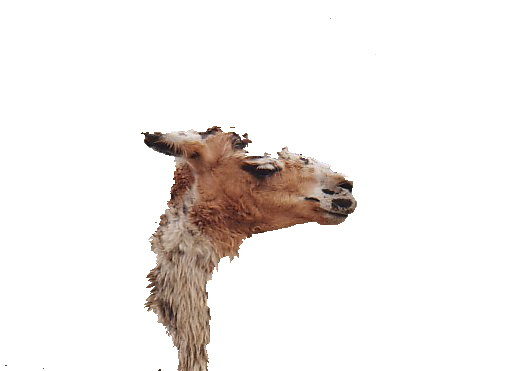
\includegraphics[width=.23\textwidth]{./figure/llama-foreground2.png}
\label{fig:graph_cut:05:foreground2} }  % smooth ratio 120
\caption{ Comparing the performance on different cases in graph cub. }
\label{fig:graph_cut:05}
\end{figure}

When the color of the foreground textile is greatly diverse, it will also hard to be extracted as expected.
An example is given in Figure \ref{fig:graph_cut:05:foreground1}.
Adding more foreground seeds manually can help the foreground extraction, as in Figure \ref{fig:graph_cut:05:foreground2}.

\bibliography{reference}
\bibliographystyle{plain}

\end{document}